\section{Results}\label{sec:results}
Both models were evaluated on the held-out test set, and the full metrics are reported in Appendix \ref{app:model_performance}. Point prediction accuracy is virtually identical: the LSTM reports an RMSE of 0.01039, and the variational GP reports 0.01038. NLL is $-3.114$ for the LSTM, and $-3.110$ for the variational GP. The LSTM achieves a higher hit rate of 54.58\% against the variational GP's 51.59\%. The variational GP is also less well calibrated, with an ECE score of 0.1135 compared to the LSTM's 0.1077. Both models converge quickly, with the best weights recovered at epoch three by early stopping (See appendix \ref{app:training_curves}).

\subsection{LSTM Network}

\begin{figure}[H]
    \centering
    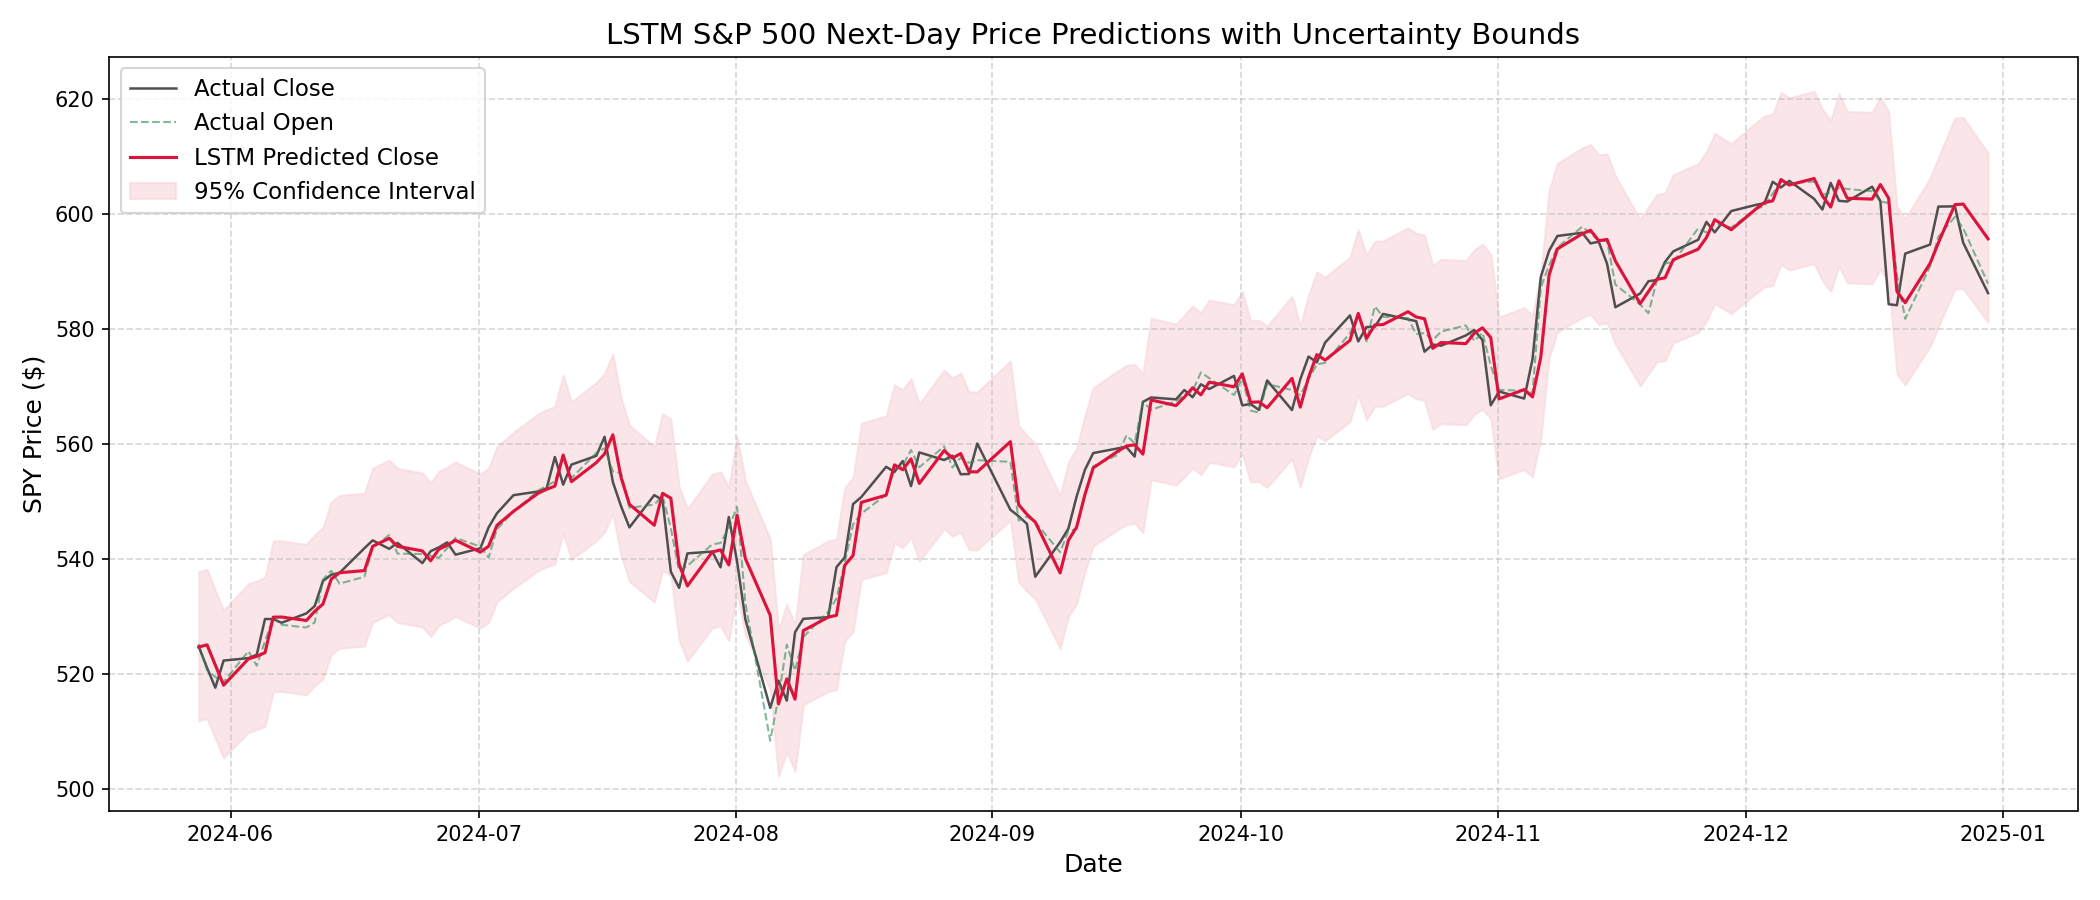
\includegraphics[width=0.8\linewidth]{overleaf/assignment_3/report/results/plots/LSTM_price_predictions.png}
    \caption{LSTM next-day S\&P 500 price predictions with 95\% confidence intervals. Predicted close prices are obtained by applying the predicted log returns to the previous day's close.}
    \label{fig:lstm_price}
\end{figure}

The LSTM tracks the general upward trend of the S\&P 500 closely at the price level, with the actual close price remaining well within the 95\% confidence band throughout (Figure~\ref{fig:lstm_price}). The band width is consistent across the period, reflecting the constant-width uncertainty in the return domain.

\begin{figure}[H]
    \centering
    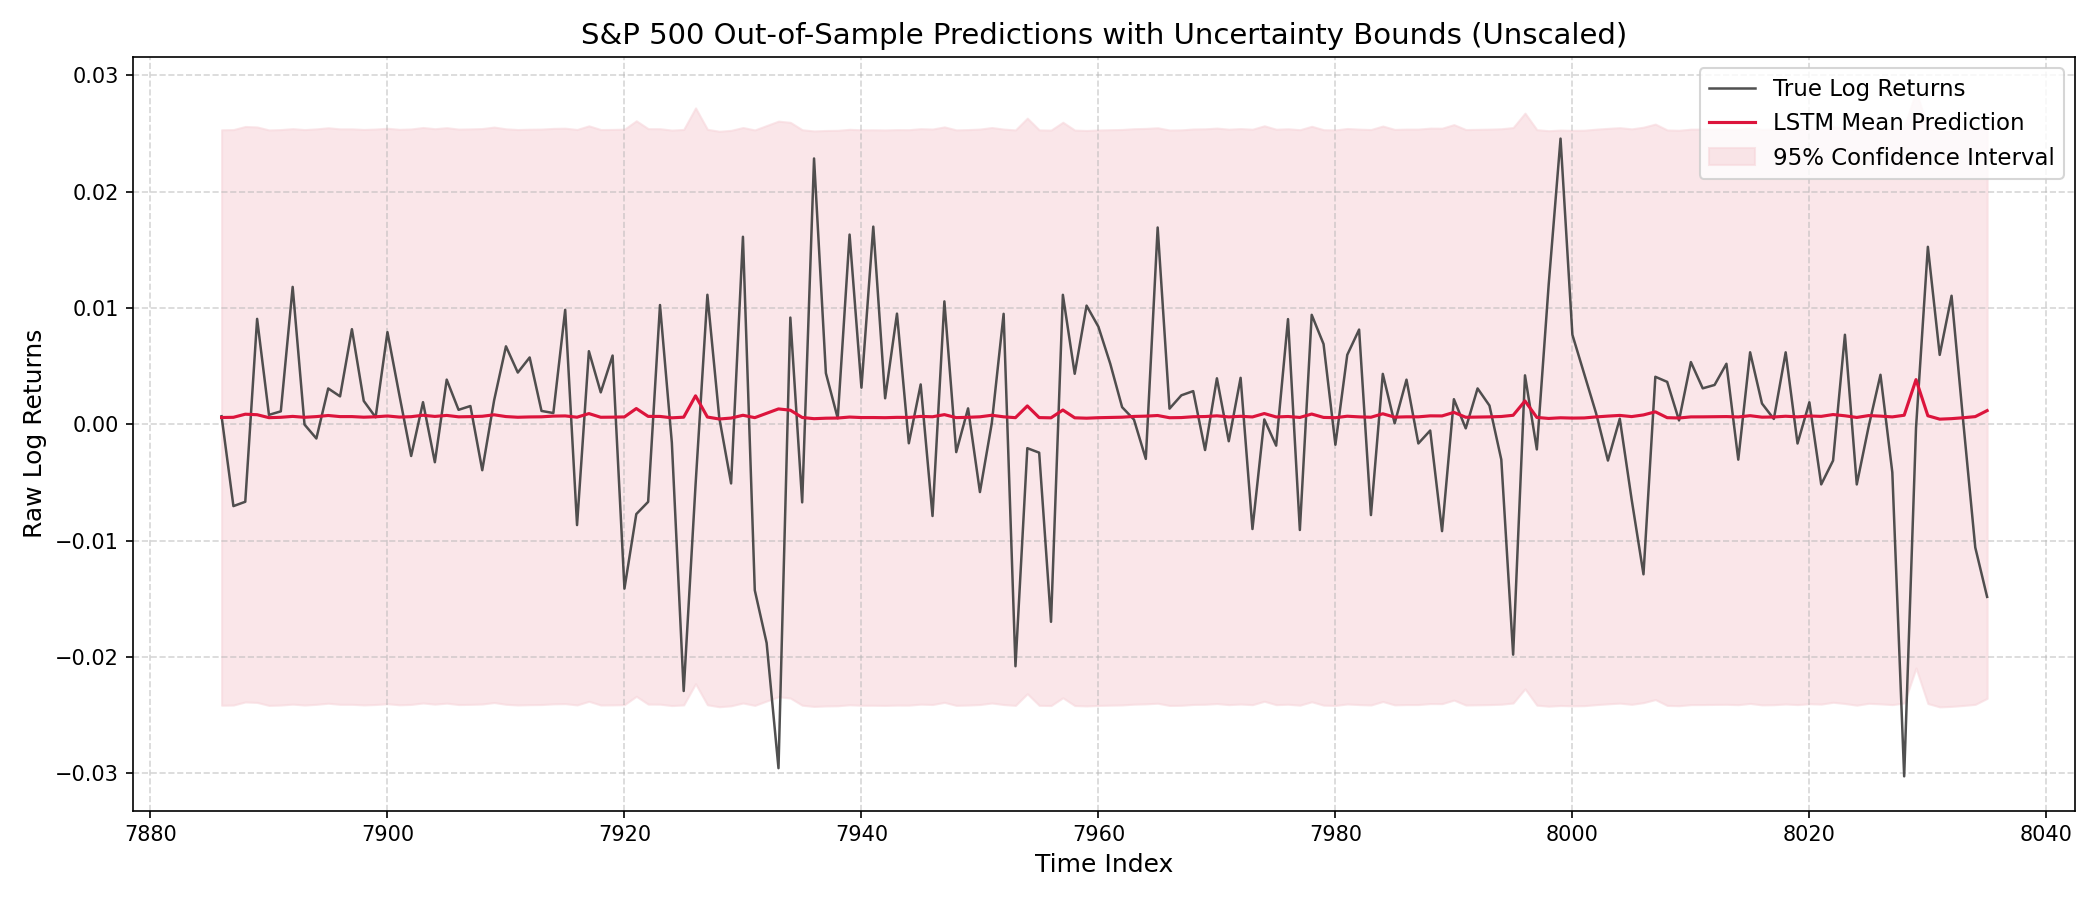
\includegraphics[width=0.8\linewidth]{overleaf/assignment_3/report/results/plots/LSTM_predictions_with_uncertainty.png}
    \caption{LSTM out-of-sample predictions with 95\% confidence intervals (MC Dropout, $N=50$).}
    \label{fig:lstm_predictions}
\end{figure}

The predictive mean stays close to zero throughout the test period, and the confidence band is wide and approximately constant in width with no visible widening during volatile periods (Figure~\ref{fig:lstm_predictions}). This suggests the MC Dropout variance is largely fixed by the architecture rather than adapting to the inputs.

\begin{figure}[H]
    \centering
    \begin{minipage}{0.45\linewidth}
        \centering
        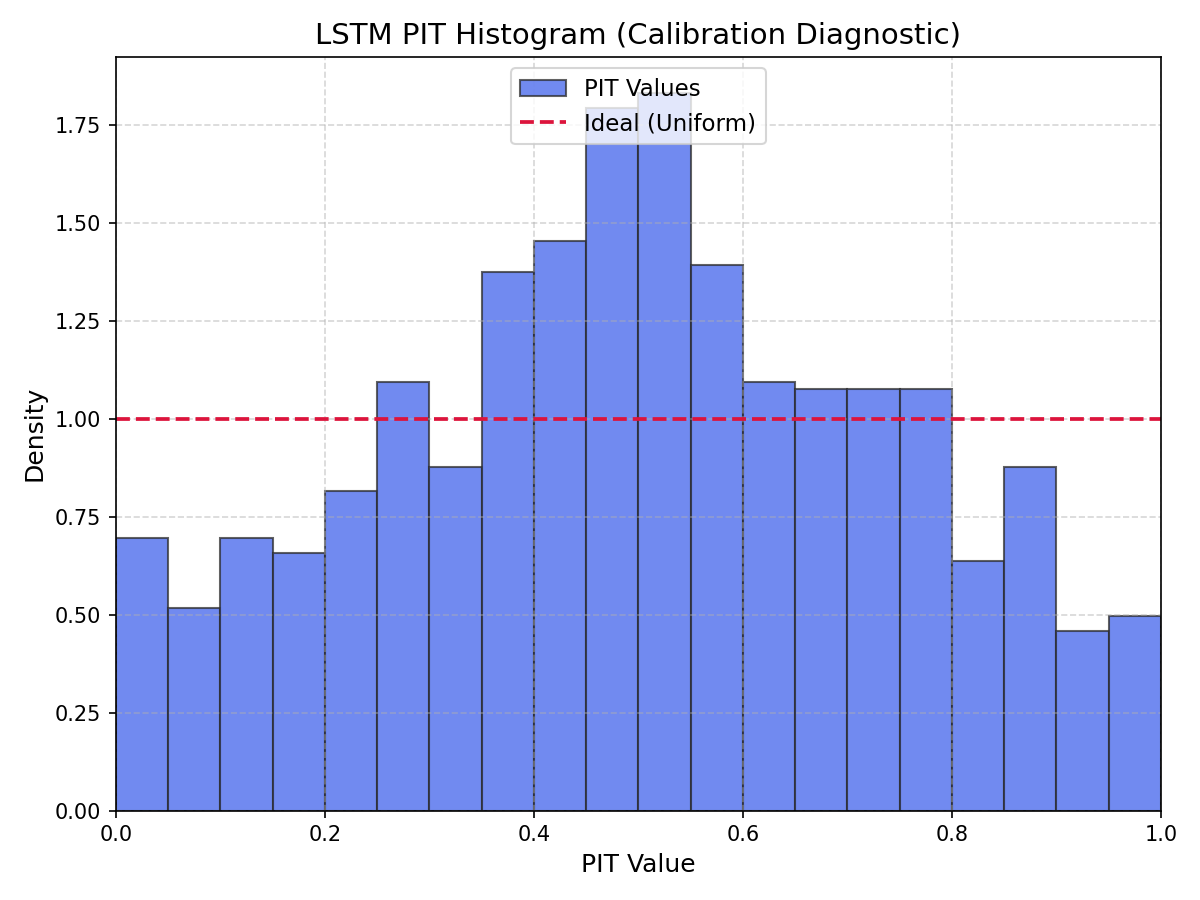
\includegraphics[height=5cm,width=\linewidth,keepaspectratio]{overleaf/assignment_3/report/results/plots/LSTM_pit_histogram.png}
        \caption{PIT Histogram.}
    \end{minipage}
    \hfill
    \begin{minipage}{0.45\linewidth}
        \centering
        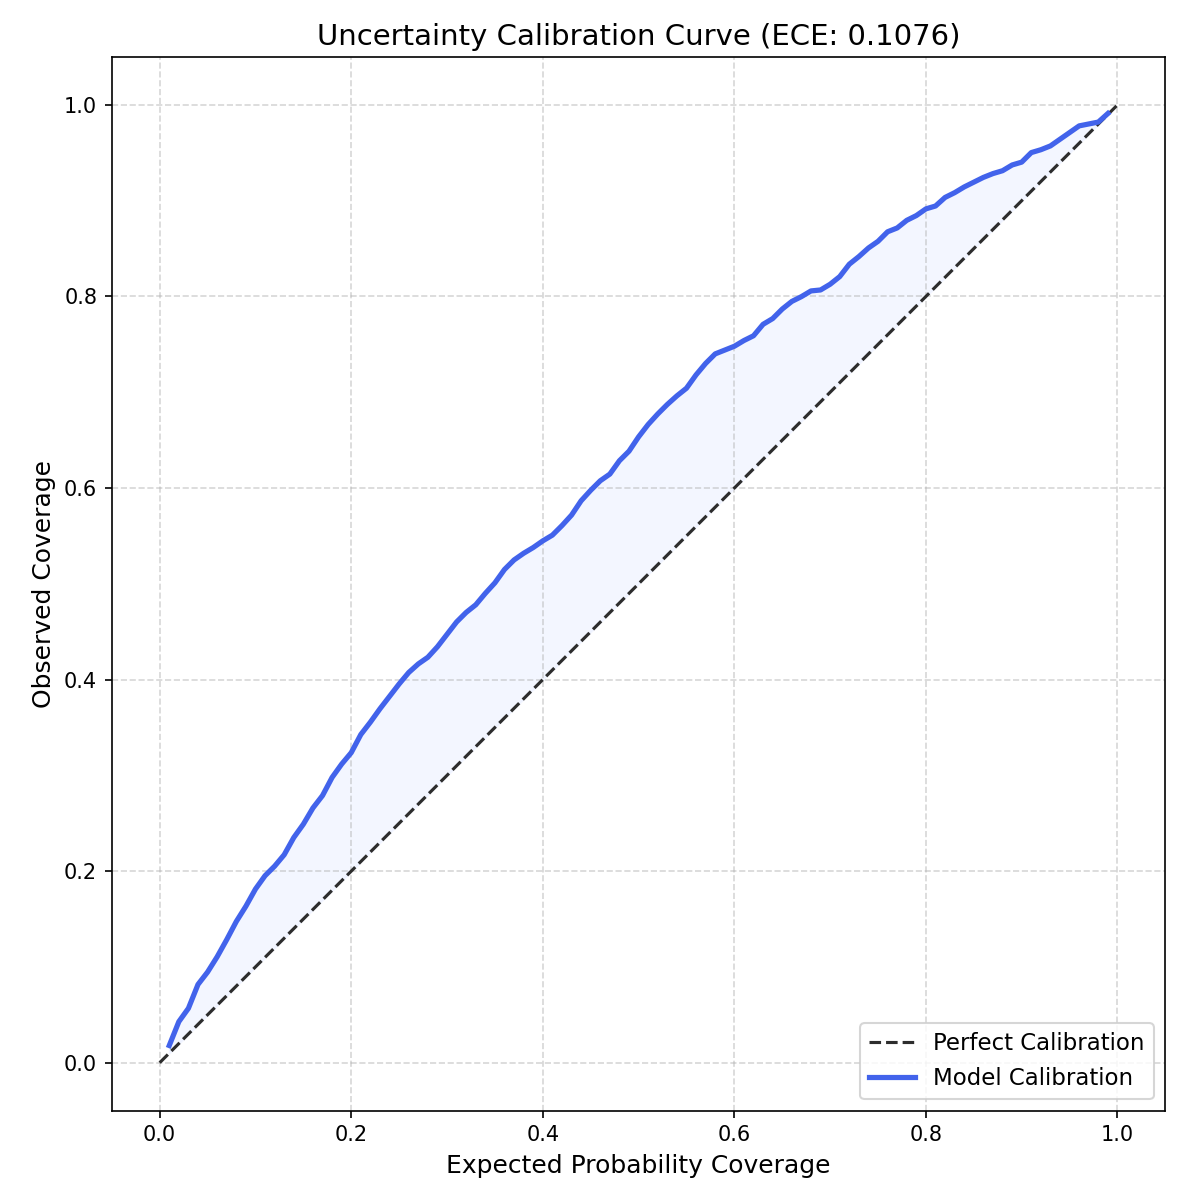
\includegraphics[height=5cm,width=\linewidth,keepaspectratio]{overleaf/assignment_3/report/results/plots/LSTM_uncertainty_calibration.png}
        \caption{Calibration Curve (ECE = 0.1077)}
    \end{minipage}
    \caption{LSTM calibration diagnostics.}
    \label{fig:lstm_calibration}
\end{figure}

The PIT histogram shows a hill shape with density concentrated around 0.4--0.6 and deficits at both tails, indicating underconfidence: the predicted intervals are wider than necessary (Figure~\ref{fig:lstm_calibration}). The calibration curve sitting consistently above the diagonal further confirms this.

\subsection{Variational GP Model}

\begin{figure}[H]
    \centering
    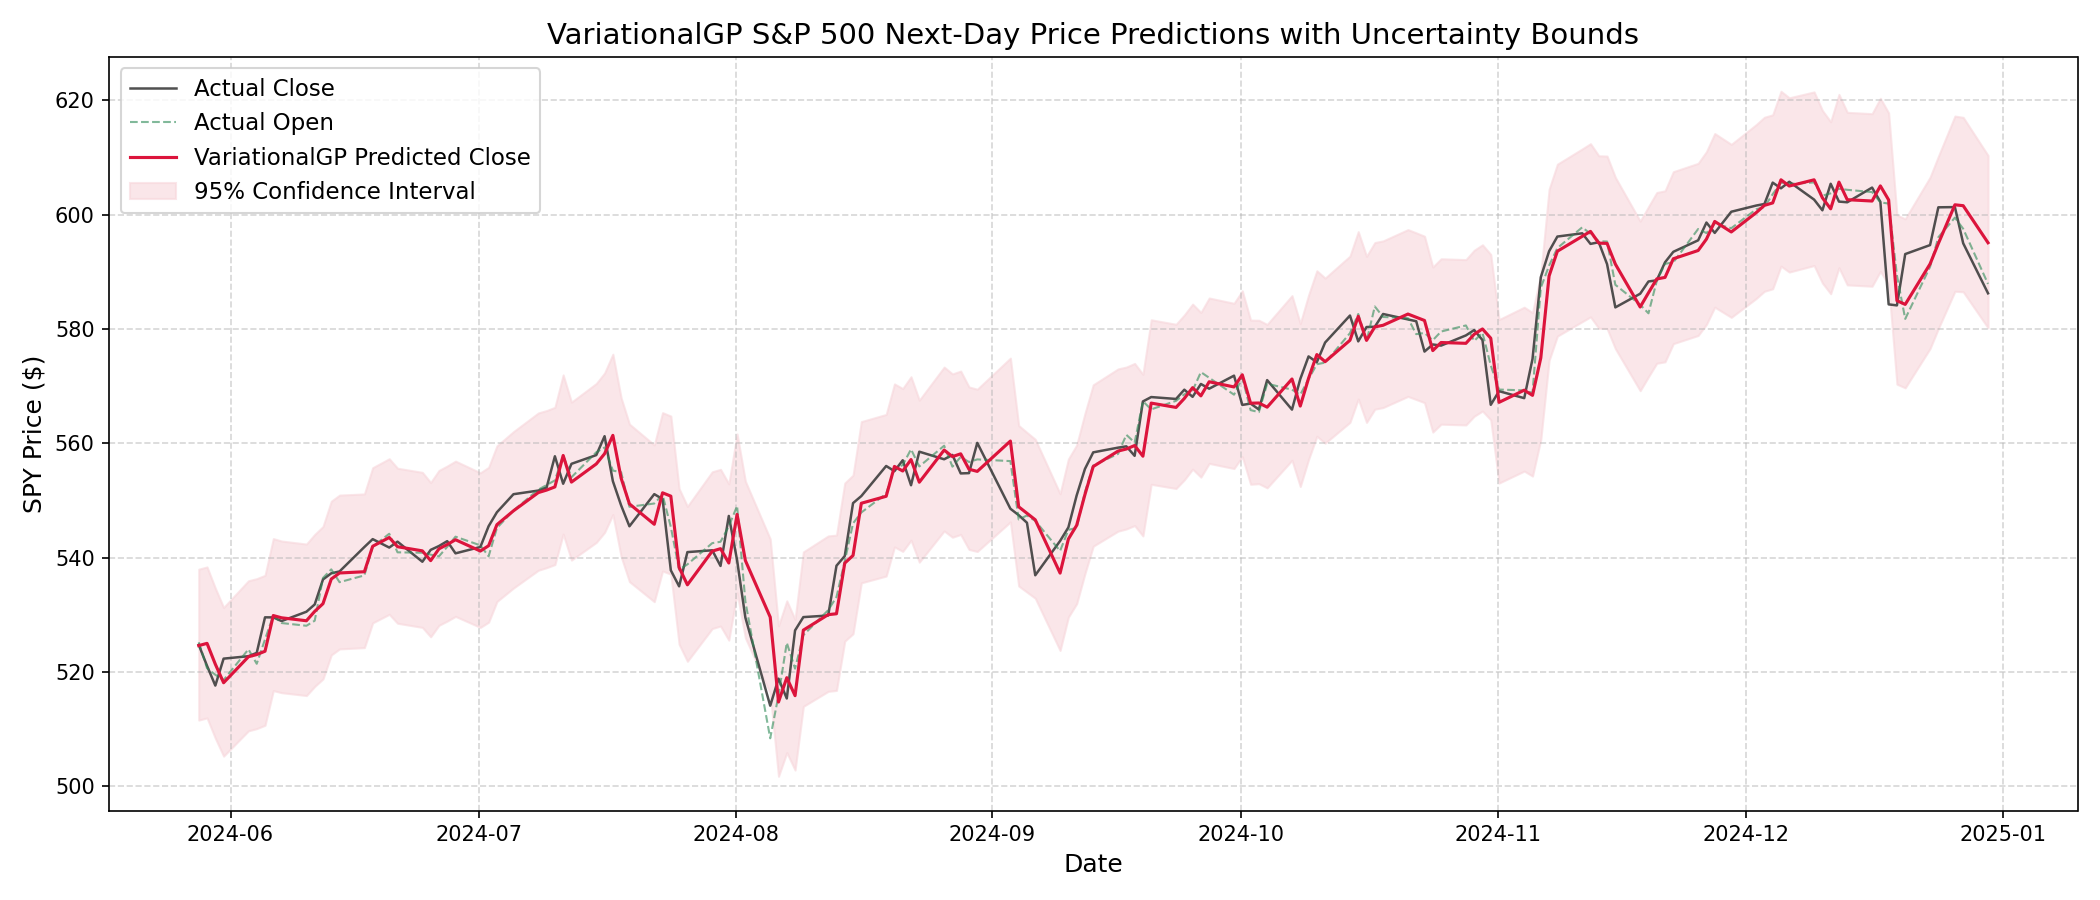
\includegraphics[width=0.8\linewidth]{overleaf/assignment_3/report/results/plots/VariationalGP_price_predictions.png}
    \caption{Variational GP next-day S\&P 500 price predictions with 95\% confidence intervals.}
    \label{fig:vgp_price}
\end{figure}

The variational GP price-level predictions are nearly indistinguishable from the LSTM's: the predicted close tracks the actual price closely, and the confidence band is wide and roughly constant (Figure~\ref{fig:vgp_price}). The similarity of the two plots is consistent with their near-identical RMSE and NLL on the test set.

\begin{figure}[H]
    \centering
    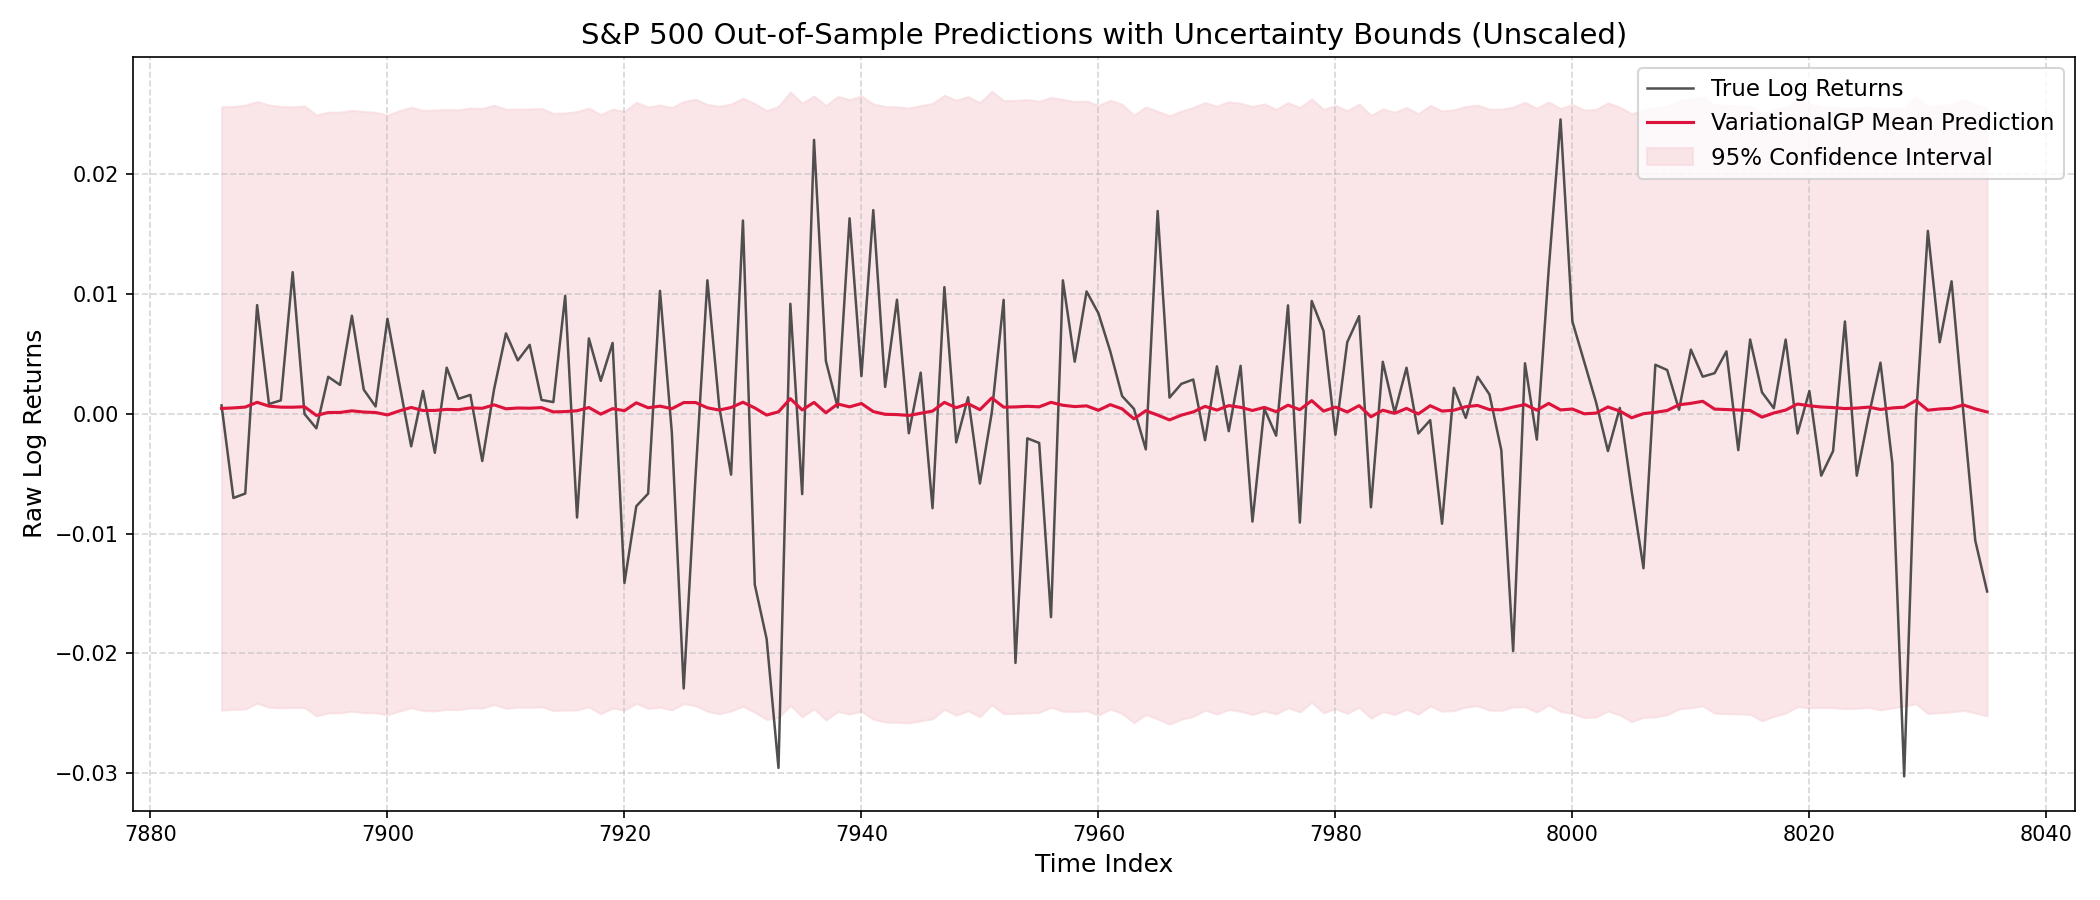
\includegraphics[width=0.8\linewidth]{overleaf/assignment_3/report/results/plots/VariationalGP_predictions_with_uncertainty.png}
    \caption{Variational GP out-of-sample predictions with 95\% confidence intervals from the analytic GP posterior.}
    \label{fig:vgp_predictions}
\end{figure}

The variational GP log-return predictions are qualitatively similar to the LSTM: a flat mean near zero with a wide, roughly constant confidence band (Figure~\ref{fig:vgp_predictions}). No regime-dependent widening is visible, which is expected behaviour from a static RBF kernel that encodes a global smoothness assumption.

\begin{figure}[H]
    \centering
    \begin{minipage}{0.45\linewidth}
        \centering
        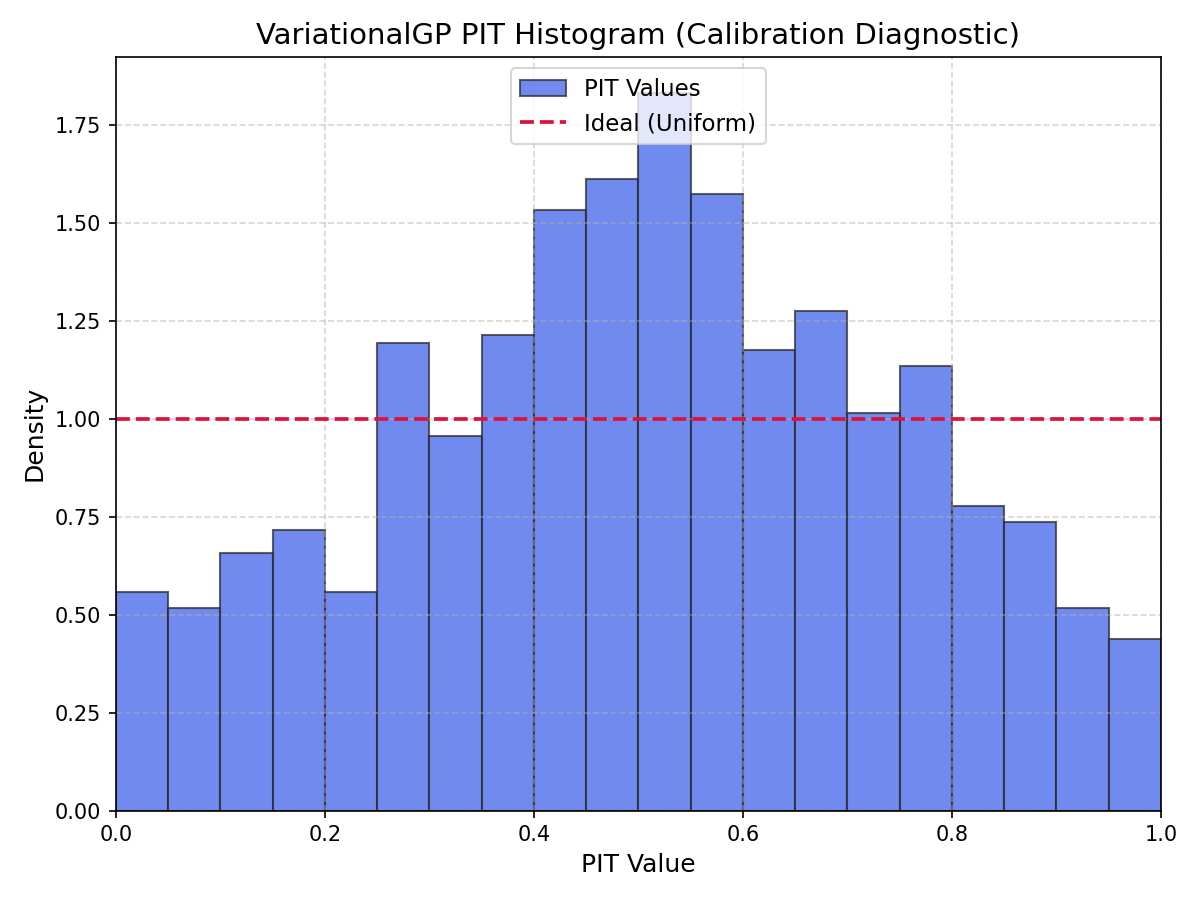
\includegraphics[height=5cm,width=\linewidth,keepaspectratio]{overleaf/assignment_3/report/results/plots/VariationalGP_pit_histogram.png}
        \caption{PIT Histogram.}
    \end{minipage}
    \hfill
    \begin{minipage}{0.45\linewidth}
        \centering
        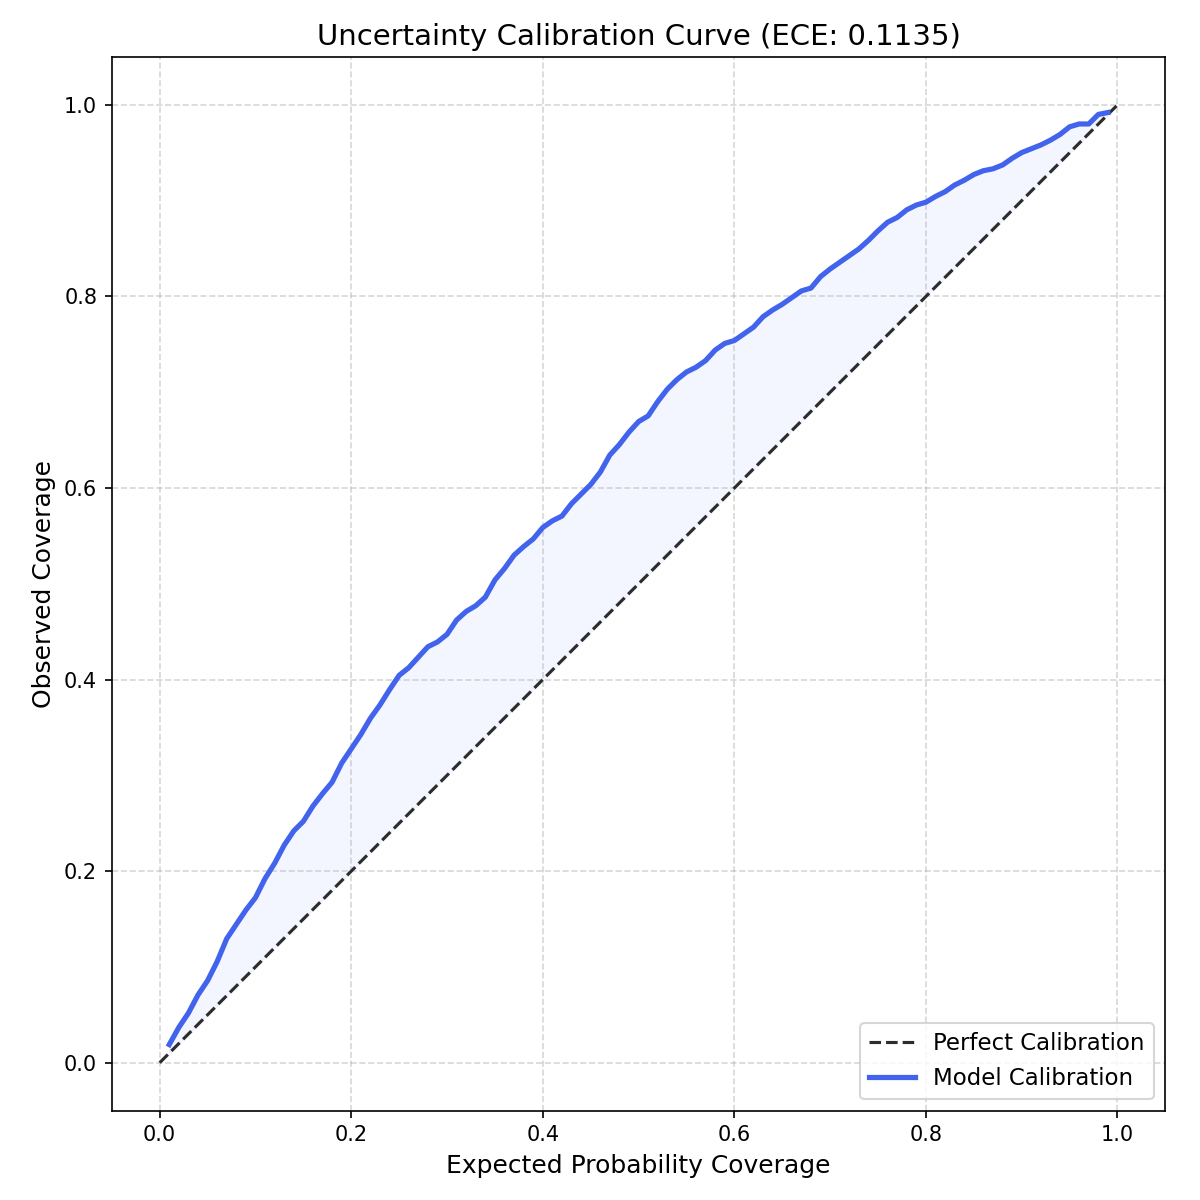
\includegraphics[height=5cm,width=\linewidth,keepaspectratio]{overleaf/assignment_3/report/results/plots/VariationalGP_uncertainty_calibration.png}
        \caption{Calibration curve (ECE = 0.1135).}
    \end{minipage}
    \caption{Variational GP calibration diagnostics.}
    \label{fig:vgp_calibration}
\end{figure}

The variational GP PIT histogram mirrors the LSTM's hill shape, indicating the same underconfidence pattern (Figure~\ref{fig:vgp_calibration}). The ECE of 0.1135 is marginally worse than the LSTM's 0.1077, meaning the variational GP's posterior variance is slightly more over-dispersed, which is again evidenced by the calibration curve sitting above the diagonal.
